\documentclass{amsart}

\usepackage{fouche}

\makeatletter
\renewcommand*\env@matrix[1][*\c@MaxMatrixCols c]{%
  \hskip -\arraycolsep
  \let\@ifnextchar\new@ifnextchar
  \array{#1}}
\makeatother

\author{}
\date{}
\title{Famiglie di funzioni}
\begin{document}
\maketitle
\noindent
Fosco Loregian \hfill A-26

La forma più generale in cui si scrive l'equazione di una conica nel piano affine è
\[\mathcal C_{\vec a}(X,Y) : a_{00} + a_{11}X^2 + a_{22}Y^2 + a_{12}XY + a_{01}X + a_{02}Y = 0\]
al variare della tupla di valori $(a_{00}, \dots, a_{22})$ in $\mathbb R^6$; la conica si può rappresentare comodamente come una matrice
\[
\begin{pmatrix}[c|cc]
  2 a_{00} & a_{01} & a_{02} \\
  \hline 
  a_{01} & 2 a_{11} & a_{12} \\
  a_{02} & a_{12} & 2 a_{22}
\end{pmatrix}
\]
e alcune quantità algebriche associate a questa matrice informano sulle proprietà geometriche della conica che definisce (per esempio, la conica è degenere se, e solo se, $\det A=0$).

La classificazione delle coniche ora si fa studiando il segno di una sottomatrice particolare, quella data dal minore $(1,1)$ della matrice in oggetto: si tratta della quantità $\Delta := -\det A' = a_{12}^2 - 4a_{11}a_{22}$, che incidentalmente coincide col discriminante del polinomio omogeneo
\[a_{11}X^2 + a_{22}Y^2 + a_{12}XY\]
ottenuto come la parte quadratica di $\mathcal C_{\vec a}(X,Y)$.

Al variare dei coefficienti in $\vec a$, la conica $\mathcal C_{\vec a}$ rappresenta i vari tipi di coniche:
\begin{itemize}
  \item Quando la conica è degenere,
  \begin{itemize}
    \item Una coppia di rette incidenti quando $\Delta \neq 0$;
    \item Una coppia di rette coincidenti quando $\Delta = 0$.
  \end{itemize}   
  \item Quando la conica è non degenere,
  \begin{itemize}
    \item un'iperbole se $\Delta < 0$; 
    \item un'ellisse se $\Delta > 0$;
    \item una parabola se $\Delta = 0$.
  \end{itemize}
\end{itemize}
Rappresentare graficamente la generica conica $\mathcal C_{\vec a}(X,Y)$ nel piano di {\tt geogebra} permette di apprezzare che il passaggio da una conica a centro a una parabola, e tra una conica a punti ellittici e una a punti iperbolici avviene con continuità nel parametro $\Delta$:
\begin{itemize}
  \item Quando $\Delta$ è negativo, si ottengono ellissi
  \begin{center}
    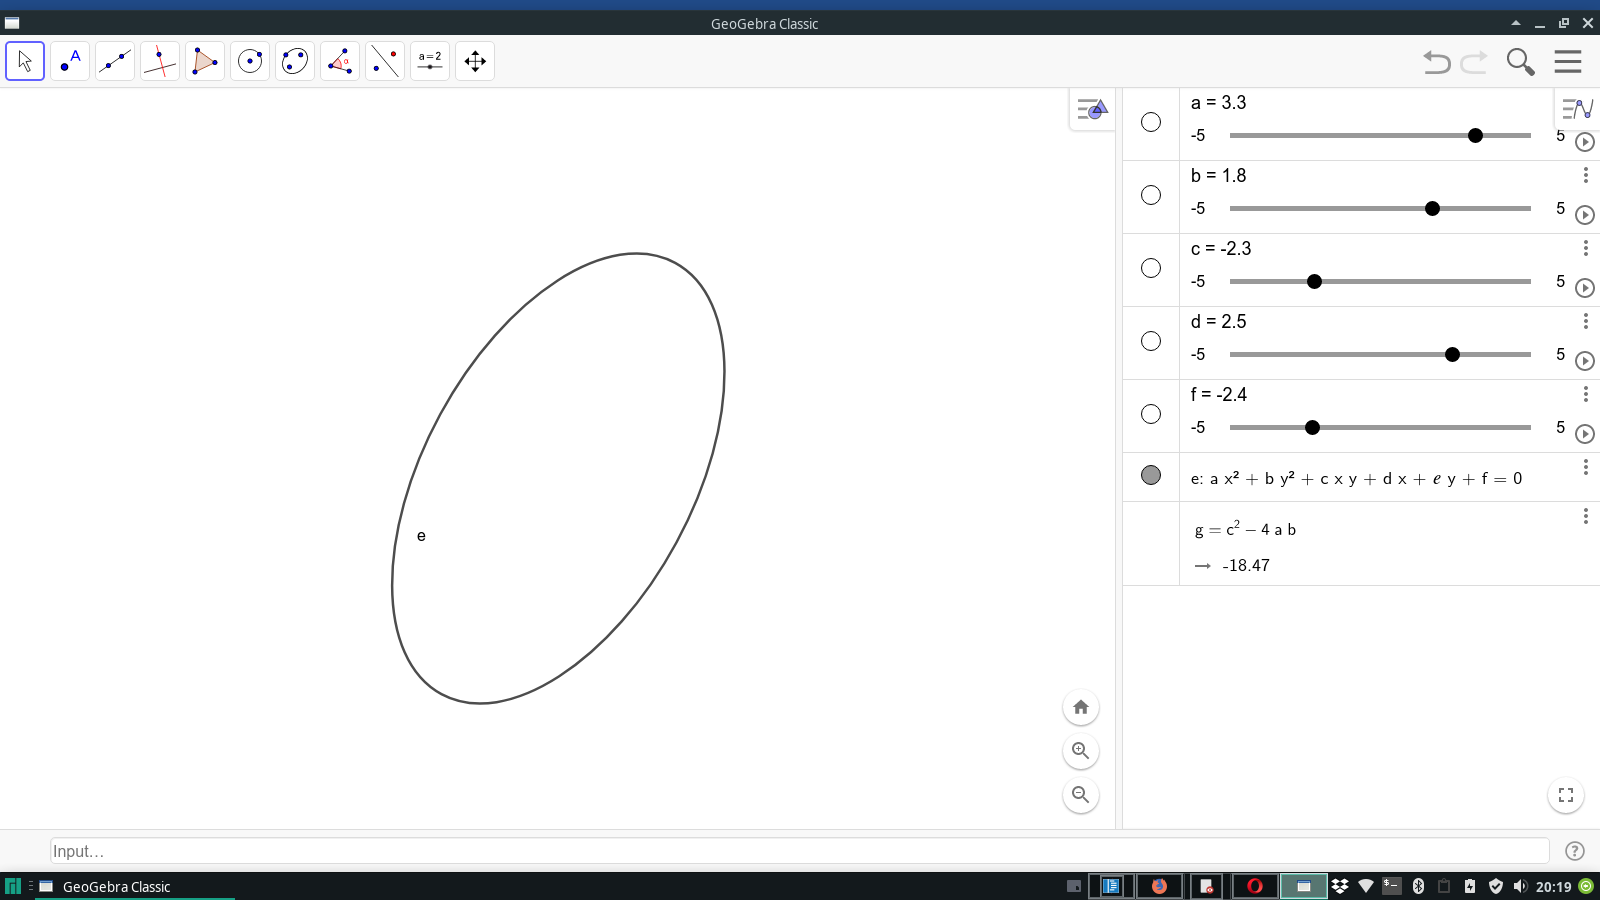
\includegraphics[width=.75\textwidth]{elly.png}
  \end{center}
  \item Per scelte peculiari dei coefficienti, per esempio $c=2, a=b=1$, si ha una parabola:
  \begin{center}
    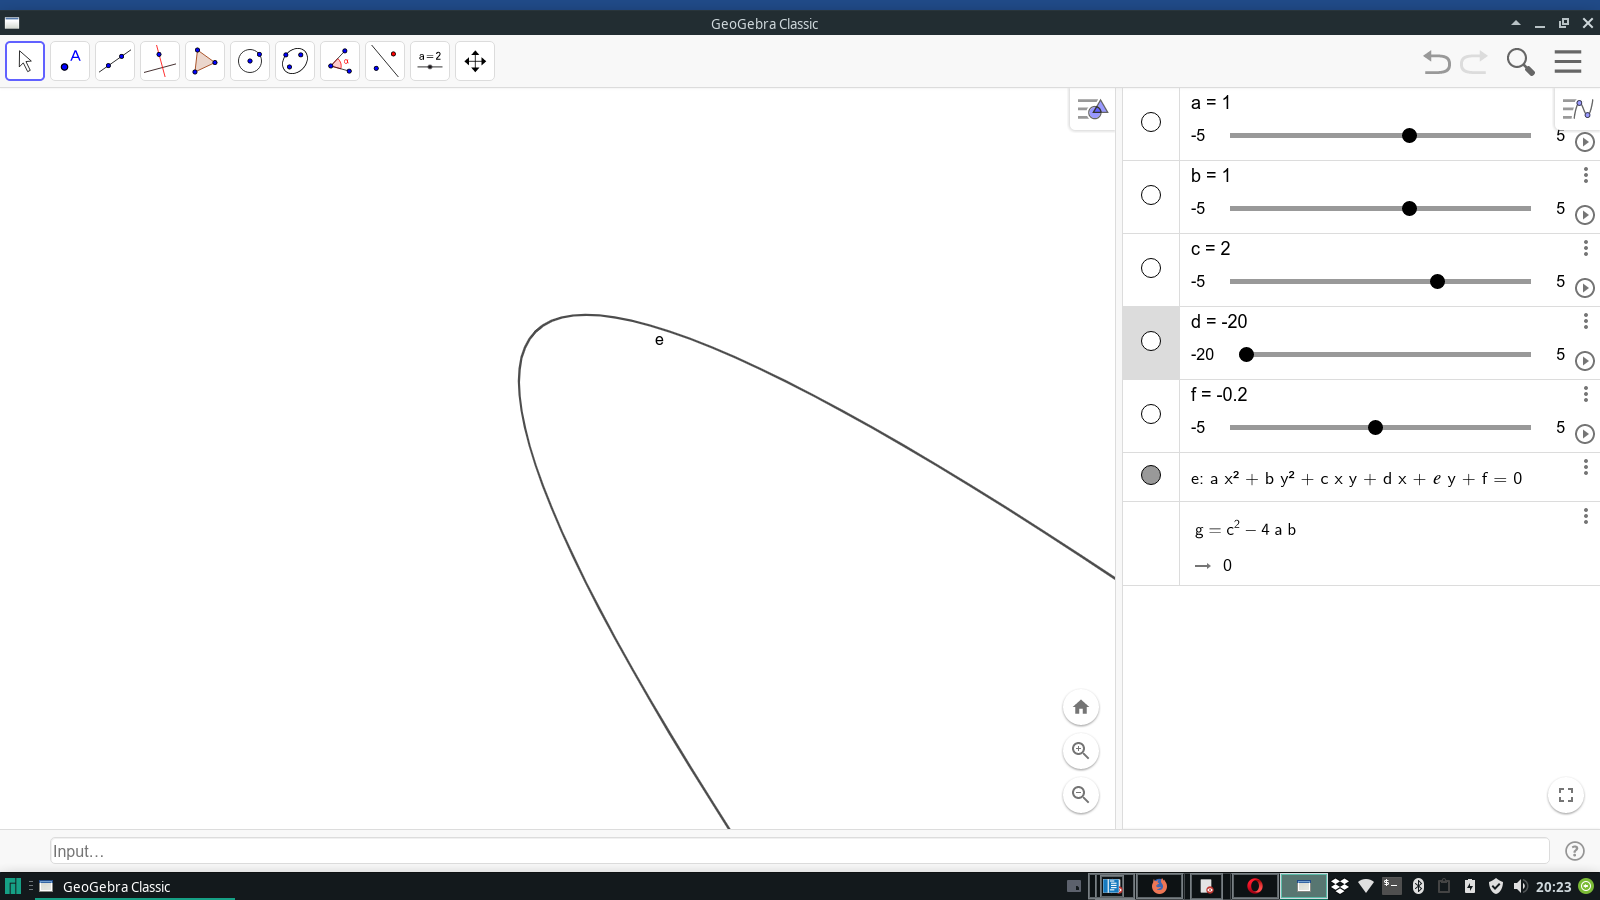
\includegraphics[width=.75\textwidth]{parab.png}
  \end{center}
  \item Quando $\Delta$ è positivo, si ottiene una famiglia di iperboli:
  \begin{center}
    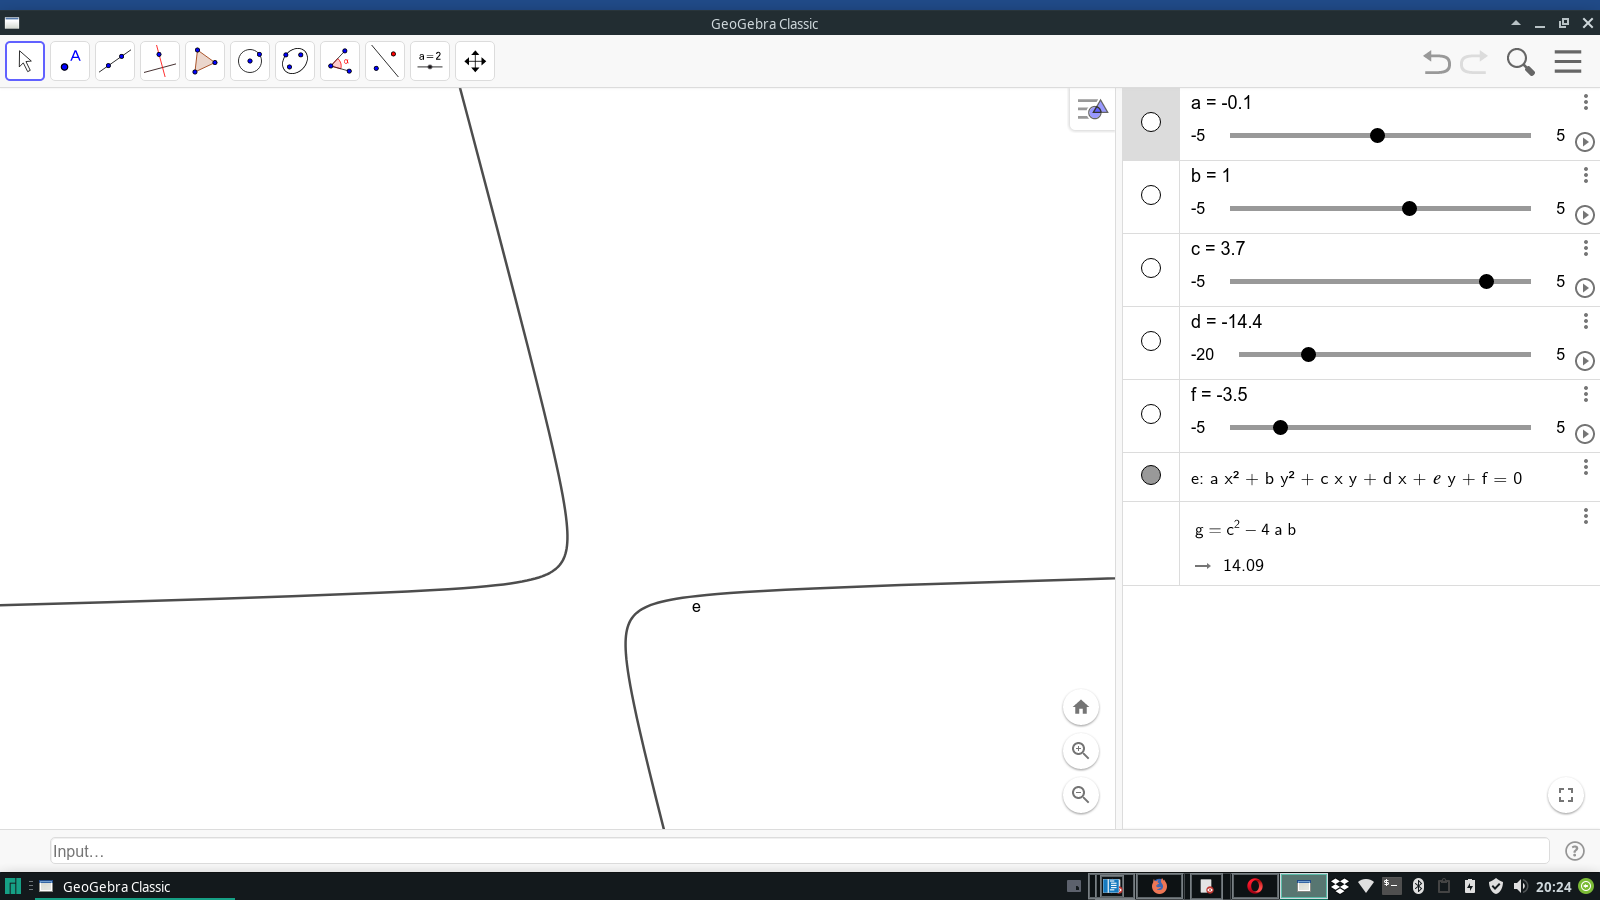
\includegraphics[width=.75\textwidth]{hyper.png}
  \end{center}
  Si può consecutivamente giocare con i parametri: per quali valori le iperboli sono equilatere? Quali coefficienti comandano l'equazione degli asintoti dell'iperbole?
\end{itemize}
\subsection{Per preparare l'attività}
\begin{itemize}
  \item Nel menu laterale selezionare {\tt View -> Input Bar}
  \item Scrivere l'equazione della conica generica nella {\tt Input Bar}
  \begin{verbatim}
    Input Bar |  a * x^2 + b * y^2 + c * x * y + d * x + e * y + f = 0
  \end{verbatim}
  {\tt geogebra} creerà gli slider all'uopo.
  \item Nel menu laterale selezionare la casella {\tt Algebra} spuntando in positivo la casella:
  \begin{center}
    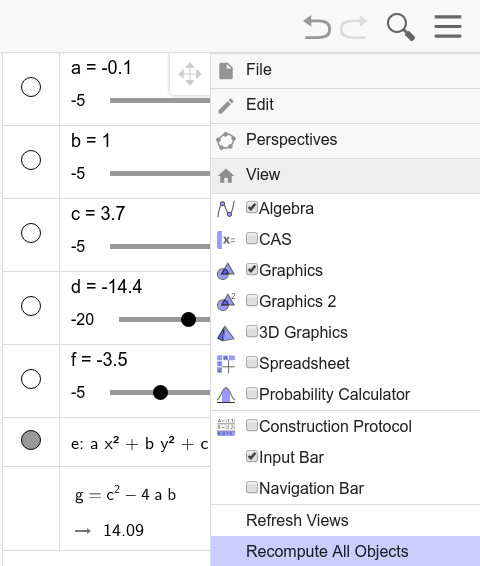
\includegraphics[scale=.2]{menubar.png}
  \end{center}
  \item Questo posizionerà gli slider nel lato destro dello schermo e permetterà di manipolarli facilmente.
\end{itemize}
\subsection{Per svolgere l'attività}
\begin{itemize}
  \item Giocare con gli slider in libertà: 
  \begin{itemize}
    \item notare che la forma della conica varia sensibilmente se si fanno variare i parametri $(a,b,c)$; 
    \item notare che lo stesso non accade se si fanno variare i parametri $(d,e,f)$: perché? Qual è la differenza tra loro?
    \item notare che il parametro $f$ trasla unicamente la conica: è ovvio il motivo!
  \end{itemize}
  \item Ora, studiare con più criterio cosa succede; trovare tre valori per $(a,b,c)$ che rendono positivo il discriminante (si otterranno quindi iperboli); inserirli a mano nella barra degli slider; si riesce a cambiare la forma della conica agendo su $(d,e)$?
  \item trovare tre valori che annullano il discriminante; inserirli a mano nella barra degli slider: si riesce a cambiare la forma della conica agendo su $(d,e)$? La figura ottenuta in questo caso è una parabola: come si calcolano a partire da $(a,b,c)$ le coordinate del suo fuoco?
  \item trovare tre valori che rendono negativo il discriminante (si otterranno quindi ellissi): come si calcolano a partire da $(a,b,c)$ le coordinate dei suoi due fuochi? (detto anche ``una parabola è solo un'ellisse con un fuoco molto molto lontano'')
  \item ``Perché'' per un'ellisse i fuochi sono due? A che condizione sui coefficienti i fuochi sono uno solo? (detto anche ``una circonferenza è solo un'ellisse che non ha mai smesso di concentrarsi'').
\end{itemize}
Da ultimo, si può visualizzare il discriminante come una ulteriore quantità
\begin{itemize}
  \item Si scrive nella {\tt Input Bar}
  \begin{verbatim}
    Input Bar |  c ^ 2 - 4 * a * b
  \end{verbatim}
  \item con ciò viene creato un ulteriore slider (che però non è associato a un oggetto geometrico);
  \item ora si osserva il risultato per i valori precedentemente scelti che rendono il discriminante positivo, negativo o nullo.
\end{itemize}
\end{document}